\documentclass[12pt, a4paper]{article}
\usepackage{amsthm,amsfonts,amsmath,amssymb,amscd}
\usepackage[T2A]{fontenc}
\usepackage[utf8]{inputenc}
\usepackage[english, russian]{babel}
\usepackage{graphicx}
\usepackage{indentfirst}
\usepackage{cite}
\usepackage{psfrag}

\IfFileExists{pscyr.sty}{\usepackage{pscyr}}{}    %

\usepackage[top=2cm,bottom=2cm,left=2.5cm,right=1cm]{geometry}

\linespread{1.3}


\begin{document}
\begin{titlepage}
\begin{center}
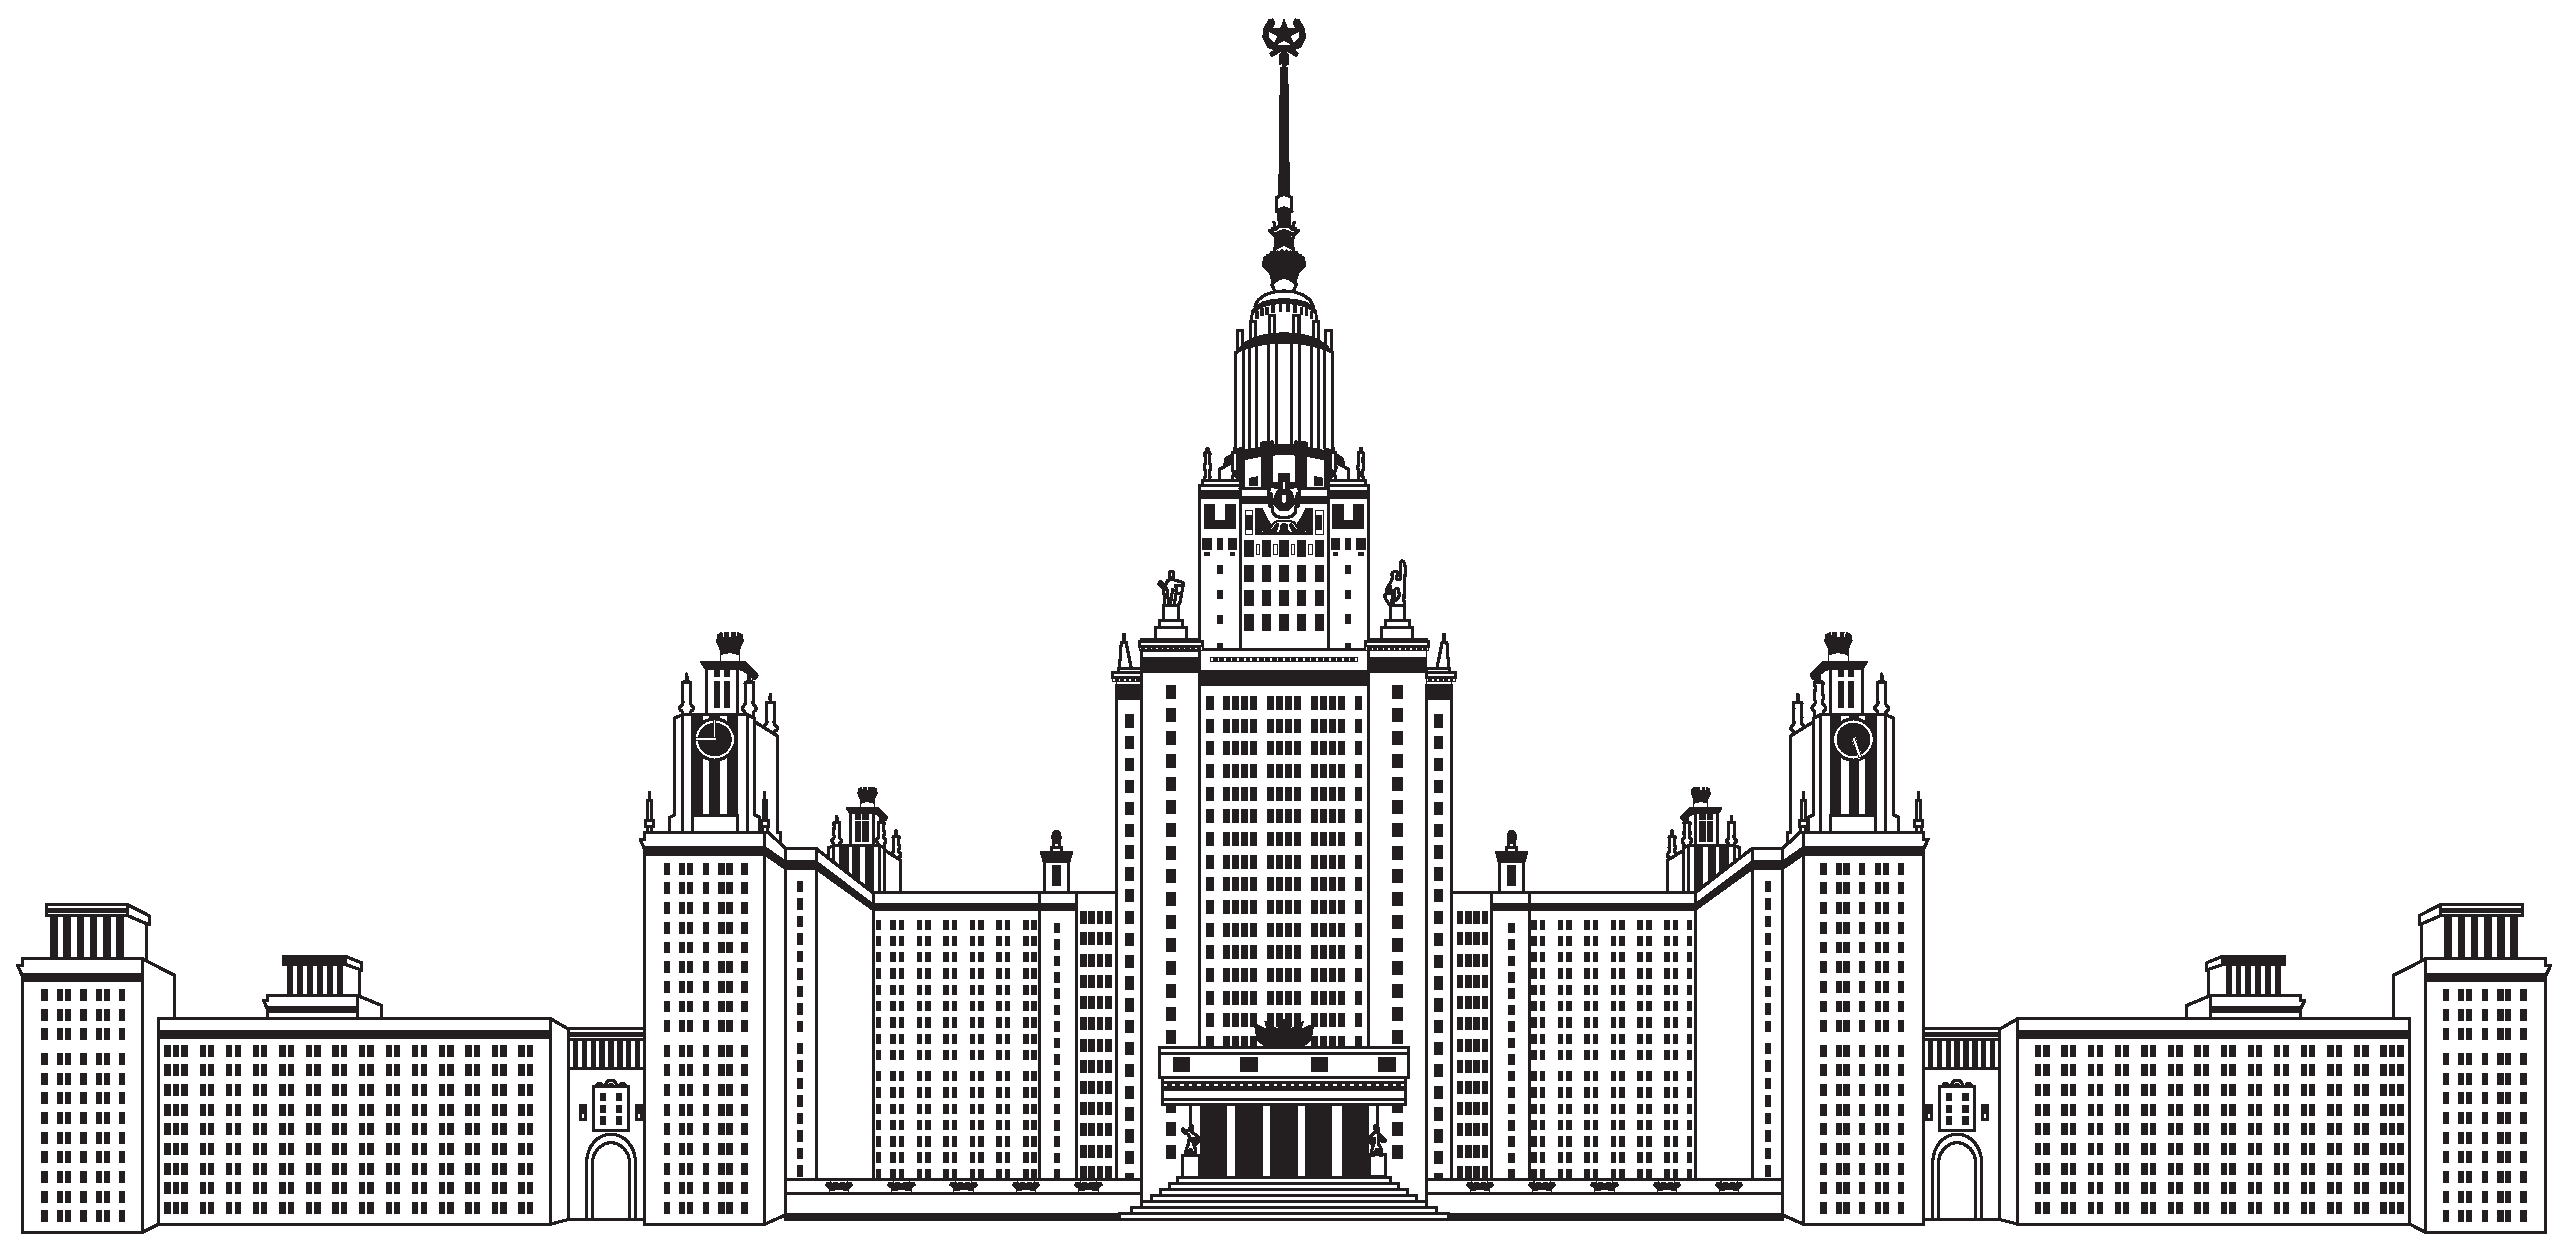
\includegraphics[width=8cm, height=4cm]{images\msu_logo}
\end{center}
\begin{center}
Московский государственный университет имени М.В. Ломоносова\\
\vspace{0.1 cm}
Факультет вычислительной математики и кибернетики\\
\vspace{0.1 cm}
Кафедра исследования операций

\vspace{3cm}
{\Large Моисеев Александр Дмитриевич }\\
\vspace{1cm}

{\bf\LARGE Кубическая регуляризация метода Ньютона}\\ \vspace{2cm}
МАГИСТЕРСКАЯ ДИССЕРТАЦИЯ

\end{center}
\vspace{2cm}
\begin{flushright}

{\bf Научный руководитель:}\\
к.ф.-м.н.\\
М.\,Р. Давидсон

\end{flushright}

 \vspace{4.5cm}

\centerline {Москва, 2018}

\end{titlepage}
\section{Введение}

\section{Постановка задачи}

\section{Заключение}

\begin{thebibliography}{30}

\bibitem{4avtora}
{\it Понтрягин Л.С., Болтянский В.Г., Гамкрелидзе Р.В., Мищенко Е.Ф.} Математическая теория оптимальных процессов. Москва. 1961. 391 с.
\bibitem{kisel_du}
{\it Киселёв Ю.Н.} Достаточные условия оптимальности в терминах конструкций принципа максимума Понтрягина.
Математические модели в экономике и биологии. Материалы научного семинара. Планерное. Московская обл.
МАКС Пресс, 2003, с. 57--67.
\bibitem{cesari}
{\it Cesari L.} Optimization — Theory and Applications. Problems with Ordinary Differential Equations. Applications of Mathematics \#17. Berlin-Heidelberg-New York, Springer-Verlag. 1983. 542 pp.
\bibitem{cost_estimation}
{\it Benson D. A., Huntington G. T., Thorvaldsen T. P., and Rao A. V.} Direct Trajectory Optimization and Costate Estimation via an Orthogonal Collocation Method. Journal of Guidance, Control, and Dynamics, Vol. 29, No. 6, November-December 2006, p. 1435-1440.
\end{thebibliography}
\end{document}
